\documentclass[a4paper, 9pt, draft]{amsart}
\usepackage[english]{babel}
\usepackage{amsmath}
\usepackage{amssymb}
\usepackage{amsfonts}
\usepackage{mathtools}
\usepackage{diagbox}
\usepackage{booktabs}
\usepackage{enumitem}
\usepackage{color}
\usepackage{hyperref}
\usepackage{tikz}
\usepackage{accents}
\usepackage{standalone}
\usepackage{bm}
\usepackage{multicol}
\usepackage{stmaryrd}
\usepackage{graphicx}
\usepackage{float}
\usepackage{syntax}
\usepackage[final]{listings}
\usepackage[font={small,sc}]{caption}

\usetikzlibrary{fit}
\usetikzlibrary{backgrounds}
\usetikzlibrary{positioning}
\usetikzlibrary{decorations}
\usetikzlibrary{decorations.pathmorphing}
\usetikzlibrary{arrows.meta}
\usetikzlibrary{chains}
\usetikzlibrary{shapes.multipart}
\usetikzlibrary{scopes}
\usetikzlibrary{arrows}


\hyphenation{block-chain block-chains}
\hyphenation{crypto-graphically}

\hypersetup{colorlinks,
    citecolor=black,
    filecolor=black,
    linkcolor=black,
    urlcolor=blue,
    pdftex}

\setlist[description]{leftmargin=1.2cm, labelindent=\parindent}
\setlist[enumerate]{leftmargin=1.2cm, labelindent=\parindent}

\newcommand*\eg{e.g.\ }
\newcommand*\ie{i.e.\ }

\title[Radicle]{Radicle}
\author{Monadic}
\date{2018}

\newcommand{\oscoin}{\textsc{\small{oscoin}}}
\newcommand{\blake}{\textsc{\small{blake2}}}
\newcommand{\hash}{\mathsc{hash}}
\newcommand{\coin}{$\Theta$}
\newcommand{\mathsc}[1]{\text{\normalfont\scshape#1}}
\newcommand{\tx}[2]{\langle \mathsc{#1}, #2 \rangle}
\newcommand{\tuple}[1]{\langle #1 \rangle}
\newcommand{\cvdots}{\multicolumn{1}{c}{\small{\vdots}}}
\newcommand{\dep}{\xrightharpoondown[e]{d}}
\newcommand{\notice}[1]{{\color{red}#1}}
\newcommand{\comment}[1]{{\color{gray}#1}}
\newcommand{\todo}[1]{\comment{\noindent\texttt{\small\emph{TODO: #1}}}}

\newcommand{\rootchain}{\gamma}
\newcommand{\State}{\mathcal{S}}
\newcommand{\state}{\mathcal{S}}
\newcommand{\Ledger}{\mathcal{L}}
\newcommand{\ledger}{\mathcal{L}}
\newcommand{\Orgs}{\mathcal{O}}
\newcommand{\apply}{\Upsilon}
\newcommand{\fold}{\Upsilon}
\newcommand{\tree}{\mathcal{C}}
\newcommand{\op}{T}
\newcommand{\env}{\rho}
\newcommand{\cont}{\kappa}
\newcommand{\mem}{\sigma}
\newcommand{\val}{\epsilon}
\newcommand{\denotation}[2]{
    \ensuremath{\mathcal{E}_{#1} \llbracket #2 \rrbracket }}
\newcommand{\denotationdesc}[3]{
    \ensuremath{\mathcal{E}_{#1} \llbracket #2 \rrbracket \env \cont \mem &= #3  }}
\newcommand{\variable}{\nu}
\newcommand{\prog}{\pi}
\newcommand{\rad}{\textsc{Radicle} }
\newcommand{\lam}{\text{\texttt{lambda }}}
\newcommand{\define}{\text{\texttt{define}}}
\newcommand{\deref}{\text{\texttt{deref!}}}
\newcommand{\mkref}{\text{\texttt{ref!}}}
\newcommand{\set}{\text{\texttt{set!}}}
\newcommand{\quotem}{\text{\texttt{quote}}}
\newcommand{\evalm}{\text{\texttt{eval}}}
\newcommand{\ifm}{\text{\texttt{if}}}
\newcommand{\stdfn}[2]{
    \texttt{#1}
    #2
    }



\DeclareMathOperator{\eval}{\Xi}

% Adjust spacing around equations. It can be a bit tight!
\expandafter\def\expandafter\normalsize\expandafter{%
    \normalsize%
    \addtolength{\abovedisplayskip}{2pt}%
    \addtolength{\abovedisplayshortskip}{2pt}%
    \addtolength{\belowdisplayskip}{2pt}%
    \addtolength{\belowdisplayshortskip}{2pt}%
}%

\newenvironment{fig}
  {\par\bigskip\noindent\minipage{\linewidth}}
  {\endminipage\par\bigskip}

% No paragraph indentation after section headers.
\makeatletter
\let\@afterindenttrue\@afterindentfalse
\makeatother

% Issue amend operator.
\DeclareMathOperator{\amend}{\times}

\newenvironment{epigraph}[2][]
{\leftskip=1cm \def\epigraph@author{#2} \smallskip\itshape}
{\par\vspace{0.5em}\normalfont\hfill---\ \epigraph@author\hspace*{0.2cm}\par\medskip}
\makeatother

% Tikz stuff

\tikzstyle{block} = [rectangle, draw,
    text width=5em, text centered, rounded corners, minimum height=4em]
\tikzstyle{line} = [draw, -latex']

\setlength{\textwidth}{\paperwidth}
\addtolength{\textwidth}{-4cm}
\setlength{\textheight}{\paperheight}
\addtolength{\textheight}{-5cm}
\calclayout

\begin{document}
\begin{abstract}
    ...
\end{abstract}
\maketitle

\setlength{\columnsep}{20pt}
\begin{multicols}{2}

\section{Introduction}
\label{s:introduction}

% Replicated state machines. Examples (Paxos, blockchains, etc.). It's purpose
% and constraints

% Variety of applications. Is there a unifying abstraction? Needs to be
% deterministic, but aside from that, a DSL-language.

% Mention radicle.

% Allows for updates that benefit from the same consistency guarantees as the
% operations themselves. Helps solve the problem of software updates in Paxos
% etc, and a more powerful form of self-amendment in blockchains. [Note that
% perfomance gains in the compiler/interpreter must happen differently, though
% separating changes that can be semantic from those that are not helps.]

% Effect system. Separating out impurity. In the case of blockchains, clients
% are *also* programmable, without sacrificing consensus.

% outline.
% Section 2) Some examples: an upgradable key-value store. A version of nomic.
% Section 3) Formal description of language.

Replicated state machines are a widely used paradigm to program fault-tolerant
systems. The paradigm involves deploying a deterministic state machine across
multiple nodes (servers); these nodes can respond to client requests, and by
agreeing on the order of these requests (consensus), ensure agreement on their
state and output. If some fraction of nodes is unavailable (or in the looser
requirement of blockchains, if they are malicious), the overall system can
still function correctly.

The service these systems replicate may be key-value stores, file-systems,
append-only logs, account balances, etc. Each of these
services is often re-implemented anew, leading to substantial development
costs, as well as subtle bugs in the interim state of the system during the
inevitable software upgrades. In this paper, we describe a language, \rad, for
defining the behaviour of replicated state machines (RSMs) independently of the
underlying consensus. The language is designed so that new domain-specific
languages (DSLs) can easily be defined for each service provided by the system.
Each such DSL is the definition of an RSM. The expressions of the DSL
are the RSMs inputs; the value such an expression evaluates to its outputs; and
the changes in the environment its state changes.

Thus, if for example the RSM we are interested
in is a ledger of accounts, expressions or inputs may be transfers, the
state may be the balance and ownership of accounts, and outputs may be the new
balances of affected accounts or an error message if the transfers are not
allowed (due to insufficient funds or incorrect permissions).

Additionally, using the same mechanism as for DSL-definition (namely, a
\emph{reflective tower}), we provide a way for upgrading the DSL itself
\emph{with the same guarantees of agreement} between nodes as the underlying
consensus, reducing the coordination difficulty of an upgrade. DSLs can be
defined in such a way that \emph{re}-definitions are themselves just one of the
sorts of inputs RSM accepts; thus nodes will agree on the ordering of the
upgrade with respect to other inputs, and will not go out of sync as a
consequence of update.

While (crucially for the purpose of ensuring consensus) the core of the language
is deterministic, \rad also possesses an additional set of primitive operations
that allow side-effects. We show how a publish-subscribe model for side-effects
(or in the formalism of \cite{Cartwright1994}, an effect-handling central which
is never provided continuations) allows responding to outputs of the state
machine or state changes in a non-deterministic way, without endangering the
determism of the state machine itself. This in turn makes the separation between
reads and writes correct by construction.

\rad has been developed in the context of a broader effort to create a
community-owned platform for open-source development (\oscoin{}), which
includes a consensus algorithm and a networking component. The \oscoin{}
platform allows users and communities to create permissioned and permissionless
RSMs with their own semantics, be it to maintain decentralized
version-controled code, issues, pull requests, or collective decision-making. \rad is
oriented towards making that process as simple and clear as possible. We do
not in this paper further discuss the broader \oscoin{} system.

In the rest of the paper, we show some example applications built with
\rad---first, an upgradable key-value store, and then more ambitiously, a game
of Nomic (Section \ref{s:examples}). We then describe the language in more
detail (Section \ref{s:language}), and compare it to other technologies.

\section{Language Syntax and Semantics}
\label{s:language}

Technologically speaking, \rad doesn't bring anything new to programming
language design. It is essentially a specific point in the design-space (and
related tooling) optimized for the following goals:
\begin{itemize}
\item[(1)] To be deterministic, so that \rad programs specifiy deterministic
  state machines.
\item[(2)] To be powerful enough to be a `universal state-machine'.
\item[(3)] To be able to restrict this power appropirately, so that malicious
  inputs can be rejected.
\item[(4)] To be concise, expressive and emphasize correctness, so that new
  chains, with new semantics can be created cheaply (in terms of development
  time), be easily understood by all participants, and hopefully be bug-free.
\item[(5')] To work well in a collaborative setting, which code being submitted
  by multiple parties in a potentially unspecified order.
\item[(5)] To have as simple as possible underlying underlying semantics, so
  that \rad interpreters are well specified, and so that \rad can be used in
  security sensitive situations.
\item[(6)] To have the ability to interpret itself, to allow chain semantics to
  be modified on-the-fly, on-the-chain.
\end{itemize}

The design-choices we made with \rad are:
\begin{itemize}
\item[(a)] It's a high-level, homoiconic LISP dialect.
\item[(b)] It has the ability to redefine a special function \texttt{eval}, which
  is used as part of its own evaluation.
\item[(c)] It has first-class functions.
\item[(d)] It's dynamically typed.
\item[(e)] It's lexically scoped with a `hyperstatic' global environment.
\item[(f)] It only has immutable values.
\item[(g)] It's has deterministic effect system for managing state (references).
\end{itemize}

LISP is well-known for being a high-level family of languages having very concise
self-interpreters, and the Scheme specification have boiled down the
semantics to a small core. Choosing a LISP helps with (2), (4) and (6), and in
particular basing the design on Scheme helps with (5).

The redefinition of \texttt{eval} is what enables (3).

Languages with first-class functions are particularly expressive, so (c) helps
with (4).

Point (d) is a compromise: it is hard to satisfy the other points (escpecially
(6)) with strong static types, even though this would help with (4). We might
try to add types in the future, but this would also inhibit the ability to
compile other-languages into \rad.

The \emph{hyperstatic} global environment means that the resolution of free
variables takes place at the definition site rather than call-site. See Section
\ref{s:hyperstatic} for explanations for how this helps with (5').

The language is kept as pure and immutable as possible, which limits
expressivity but emphasizes clarity and correctness (goal (4)). The abundance of
mutability would also probably hinder (5').

Since chains are inherently stateful, we felt that the inclusion of a reference
type for managing state would help in the specification of chain semantics.
However we will discuss the alternatives.

The rest of this section goes into the details of these goals and
design-choices.

%% \rad is a a Lisp dialect. It uses prefix parenthesized function application,
%% supports recursion, has first-class functions, is dynamically typed, and
%% homoiconic. It differs from most Lisps in a few aspects, described below.

%% Like most Lisps, binding is lexical. Unlike most Lisps, Like Clojure, \rad
%% emphasises immutability, and mutable values must be created, read, or written
%% with specific functions (\texttt{ref}, \texttt{read-ref}, and
%% \texttt{write-ref}, respectively).


\subsection{LISP}

A minimal Scheme has the particularity that a minimal interpreter of itself can
be implemented in a few lines of code. This is achieved by:
\begin{itemize}
  \item Code being represented by the core data-structures of the language.
  \item The language being built up by a very small set of primitives: a few
    special forms and some primitive functions.
\end{itemize}
Let's consider a basic example of a chain which might want to change a part of
its semantics. In chain $C$ participants may \texttt{boot} certain other
participants, if some condition is met, which is defined by a predicate
\texttt{bootable?}. For example, \texttt{bootable?} might be defined as:
\begin{verbatim}
(define bootable?
  (lambda (a p)
    (and (admin? a) (not (admin? b)))))
\end{verbatim}
That is, admins may boot non-admins. At some point the participants may decide
that this is too crude, and that a participant should only be booted if the
majority of participants agree. For the change to take place, most likely one of
the inputs to the system will contain code for a new version of
\texttt{bootable?} (the semantics of when such a message is to be accepted would
probably be defined by yet another predicate). This code must be transmited and
interpreted in the simplest and and most transparent way possible. By choosing a LISP,
this code is carried by simple data-structures and the interpretation process is
very direct (skipping parsers, complicated abstract syntax trees, etc.). This
gives the participants better confidence in understanding what the current and
proposed semantics are.

\subsection{Hyperstatic Environments}
\label{s:hyperstatic}

Most scripting languages are intended for programs where the developer can
decide exactly where code should be placed, and be fully aware of the context
that precedes it. One can always add a line \texttt{y = bar(x)} immediately
\emph{after} \texttt{x = foo(3)}, and not worry that perhaps something else was
added in between that changes what \texttt{x} is (excepting pathological cases
of distributed code collaboration).

This is not true in the environment \rad is intended to run. In that
environment, users submit individual expressions or declarations to a running
system that is \emph{at the same time} also accepting inputs from other
users. Moreover, the view of the program that the submitter has at the time of
submission may \emph{already} be outdated. This aspect is even more significant
in the context of a blockchain, where expressions are queued until a block is
created by a node, but what those expressions in the queue are is not
accessible to other nodes.

This fact may lead to bugs or attacks. Consider the following snippet:

\begin{verbatim}
(define transfer (lambda (from to amount) ...))
(define account-alice ...)
(define account-bob ...)
(define transfer-to-alice (lambda (from amount)
  (transfer from account-alice amount))
\end{verbatim}

A user now wants to transfer some amount to Alice. However, in a language such
as Scheme the function call \texttt{(transfer-to-alice account-bob 10)} may
behave differently than this snippet alone indicates in two ways. First,
\texttt{transfer-to-alice} and \texttt{account-bob}, which explicitly appear in
the expression being submitted, may be shadowed by a new definition. Second, the
variables \texttt{transfer}, \texttt{account-alice}, and \emph{any other} free
variables used in the body of \texttt{transfer} or transitively, in the function
bodies of the functions \texttt{transfer} calls, may have been redefined.

One solution is to not allow the redefinition of variables at all. This is
indeed what some smart contract languages do, and can easily be implemented in
\rad as well (see Section \ref{s:reflective-towers}). But this comes with its
own problems; one cannot define an improved version of a function that shadows
the old one, and must instead accept a more and more polluted environment (which
additionally may impact memory usage).

An alternative is to have a mechanism to make expressions invalid if any of the
variables they rely on have been redefined since a specified line of code.
However this option is quite severe. Consider:

\begin{verbatim}
(define x 3) ;; line 1
(define foo (lambda () x)) ;; line 2
(define x 5) ;; line 3
\end{verbatim}

The function call \texttt{(protect-at-line 2 (foo))} will fail despite having a
perfectly reasonable interpretation - namely, \texttt{(foo)} \emph{with}
\texttt{x} \emph{as if used after line 2} (i.e., with \texttt{x} being
\texttt{3}). For more complex expressions, which may rely on many variables,
this problem becomes more significant.

This reasonable interpretation is in fact precisely what hyperstatic
environments provide. The function call \texttt{(foo)} in line 4 would, in this
model, still evaluate to \texttt{3}. The free variables of a function refer to
the values of variables \emph{when they were defined}. This is the semantics
\rad adopts in general (and can be found in some other languages, such as
Forth).

Now \texttt{(protect-at-line (foo))} may be given a much simpler definition:
\texttt{(foo)} if \texttt{foo} \emph{alone} has not been redefined, and otherwise
an exception. If \texttt{x} has been redefined, that is no matter, since it
anyhow does not change the meaning of \texttt{foo}.

%%% End section

\subsection{\texttt{eval} redefinition}

\rad should be able to emulate any state machine. Of course most state-machines
don't accept arbitrary inputs, and certainly not inputs which change the
semantics of the state-machine. Thus \rad should have some built in mechanism
for controlling how inputs get interpreted. At the start inputs are sent
directly for evaluation by the `base' evaluator, so it's natural to associate
modifying this process with redefining a function which represents evaluation.
When taken to the extreme, \emph{all} evaluation is done with a call to the
special function \texttt{eval}, and this creates a reflective tower of
interpreters. In \rad, a more limited form of \texttt{eval}-redefinition is
available, which only takes effect on the next input. As an example:
\begin{verbatim}
> (define eval (lambda (expr) 3))
=> ()
> 5
=> 3
\end{verbatim}

Contrast this with the sort of \texttt{eval}-redefinition that is available in the language Black:
\begin{verbatim}
(exec-at-metalevel
  (let ((old-eval base-eval))
    (set! base-eval
          (lambda (exp env cont)
            (write exp) (newline) (old-eval exp env cont)))))
\end{verbatim}
After this the Black REPL will behave as follows:
\begin{verbatim}
> (+ 1 2)
(+ 1 2)
+
1
2
=> 3
\end{verbatim}
Note in particular that the new evaluation function is used recursively, at all
levels of the expression \texttt{(+ 1 2)}.

Compare this to the following \rad session:
\begin{verbatim}
rad> (define eval (lambda (e) (do (print! e) (eval e))))
=> ()
rad> (+ 1 2)
(+ 1.0 2.0)
=> 3.0
\end{verbatim}
First of all note that we do not need to create a binding to the previous
version of eval; because of the hyperstatic environment the symbol \texttt{eval}
in the new definition of \texttt{eval} always refers to the old version of the
evaluation function. Second, in Black, \texttt{old-eval} calls out to
\texttt{base-eval}, and in subsequent evaluation this will refer to the new
definition. This is what makes the new evalution behaviour take effect at all
levels of evaluation. In \rad, the new evaluation only gets invoked at the
topmost level, on new inputs. If one wants to make the evaluation behaviour
recursive this has to be coded explicitely.

In most cases chains will define a domain-specific language to be interpreted in
some narrow way, with only some calls to the base eval to reify function
definitions, in case one wants to modify the behaviour of the state-machine in
some way. Furthermore, this form of evaluation redefinition doesn't (by default)
create a tower of interpreters. Evaluating in a towers requires advanced
interpretation methods otherwise performance suffers greatly, and this is all
the more important in \rad's case where chains may be very long-lived. Such
methods are still the subject of active reasearch, and may interfere with other
requirements of the language. For these reasons we beleive that this limited
form of eval-redefinition suits the needs of \rad better than the sort of
reflection that can be found in languages such as black.

%% \rad does not have macros. Instead, it allows for a complete redefinition of
%% the intepreter via redefinitions of \texttt{eval}.

%% \begin{verbatim}
%% (define eval (lambda (expr) 3)) ;;
%% 5 ;; => 3
%% \end{verbatim}

%% This enables users to very easily define sublanguages for new chains, or amend
%% the language running in the current one.

For a more involved example, consider a simplistic key-value store:

\input{out/kv0.rad-tex}

After which we have:

\begin{verbatim}
> (set key1 3)
=> ()
> (get key1)
=> 3
> (+ 3 2)
=> 'invalid-command

;; Note that nested expressions are not evaluated:
> (set key2 (+ 3 2))
=> ()
> (get key2)
=> '(+ 3 2)
\end{verbatim}

% TODO: maybe move to Related Work section
\subsection{Connection to Reflective Towers}
\label{s:reflective-towers}

The \texttt{eval}-redefinition mechanism resembles prior work on
\emph{reflective towers}. A reflective tower is an infinite sequence of
interpreters (called `levels') $L_0$, $L_1$, ..., where level $L_n$ is
interpreted by $L_{n+1}$. Reflective towers allow both \emph{reification}---the
ability to inspect a computation via constructs of a higher level---and
\emph{reflection}, that is, the ability to define and enter new, lower levels.
Conceptually, \rad differs from reflective towers by only allowing reflection.
Thus, the only levels that exist are the ones programs create. Queinnec has
quipped that reflective languages ``plunge us into a world with few laws, and
hardly any gravity''\cite{Queinnec1994}; the more disciplined approach to
reflection that \rad takes does not possess the semantic fragility of modifying
meta-meta-intepreters.

The techniques that have been developed for reducing the interpretive overhead
of such towers of interpreters, however, still
apply (see, for example, \cite{Amin2017}, \cite{Asai2014}), as do simpler
partial-evaluation-based approaches such as \cite{Brown2017}.

\subsection{Immutable values and refs}
In \rad all values are immutable: once created they cannot be modified in any
way. This follows in the footsteps of languages such as functional programming
languages such as Haskell, Clojure, Erlang, etc.

TODO: talk about how this leads to more correctness, and also how mutation would
be all the more confusing in a collaborative coding environment (same sort of
arguments as why mutation is hard in multi-threaded code).

However state-machines are inherantly stateful, so a reference type is included
in the language.

TODO: explain

Other things we might have consider, or might consider in the future: Another
possibility is to have an single implicit global state (essentially a single
predefined ref), and for computations with this state to be formulated using a
state-monad. Having only a single location for holding state might encumber the
developer, but providing a nice interface to state manipulation using lenses
might make this a viable option.


\subsection{Effects} In order to maintain determinism and safety in on-chain
computations, and at the same time be a useful language for scripting
interactions with chains, \rad keeps a separate, \emph{impure} environment,
$\rho_{!}$ (these are by convention textually distinguished by identifiers
ending with an exclamation mark). Expressions on chain therefore cannot have
side-effects; instead, they may evaluate to a value that \emph{describes} an effect,
but the decision of whether or how to actually carry on that effect happens at an
effect-handling layer. This architecture, with a central authority
administering effects received via messages, resembles work following
\cite{Cartwright1994} and \cite{Bauer2003}.


\begin{figure}[H]
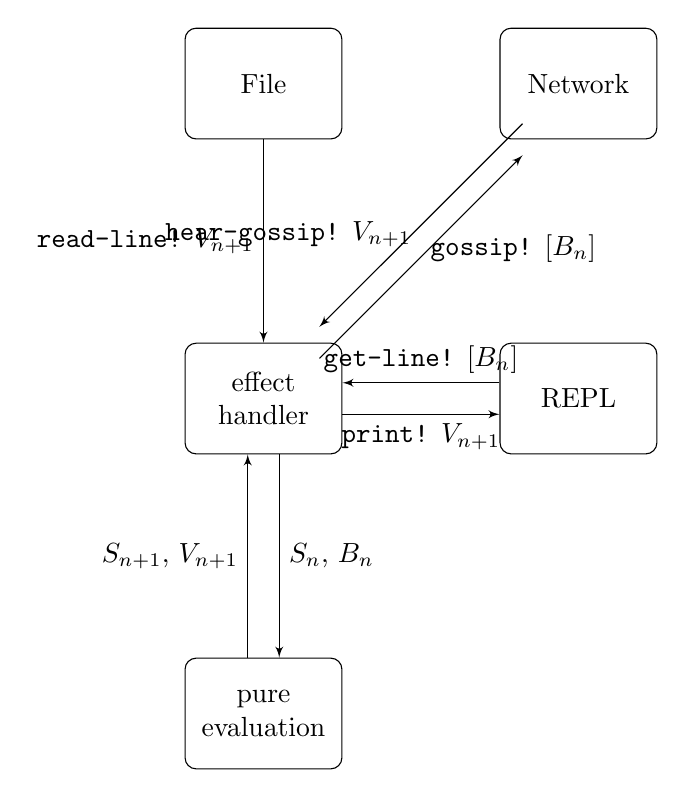
\begin{tikzpicture}[node distance = 4cm, auto]
  \node [block] (net) {Network};
  \node [block, below of=net] (repl) {REPL};
  \node [block, left of=repl] (impure) {effect handler};
  \node [block, below of=impure] (pure) {pure evaluation};
  \node [block, above of=impure] (file) {File};

    \path [line]
    (file) -- node [left] {\texttt{read-line!} $V_{n+1}$} (impure);

    \path [line, transform canvas={yshift=0.2cm}]
    (net) -- node {\texttt{gossip!} [$B_n$]} (impure);
    \path [line, transform canvas={yshift=-0.2cm}]
    (impure) -- node {\texttt{hear-gossip!} $V_{n+1}$} (net);

    \path [line, transform canvas={yshift=0.2cm}]
    (repl) -- node [above] {\texttt{get-line!} [$B_n$]} (impure);
    \path [line, transform canvas={yshift=-0.2cm}]
    (impure) -- node [below] {\texttt{print!} $V_{n+1}$} (repl);

  \path [line, transform canvas={xshift=0.2cm}]
    (impure) -- node {$S_n$, $B_n$} (pure);
  \path [line, transform canvas={xshift=-0.2cm}]
    (pure) -- node {$S_{n+1}$, $V_{n+1}$} (impure);

\end{tikzpicture}
\caption{Effect system}
\label{f:effects}
\end{figure}

The value that results from evaluating an expression purely may, in addition to
\emph{describing} an effect, pass a continuation with the result of that
effect (if any). The effect-handling layer can chose to only call continuations
without arguments. This in turn means the continuation will not have access to
the result of effectful computations, though it may (at the discretion of the
effect-handling layers) have output effects.

\begin{figure}[H]
\input{out/repl.rad-tex}
    \caption{A simple effect handler. The function \texttt{subscribe-to!}
    repeatedly calls the \texttt{getter} key of its first argument, handling
    effects with its second argument. \texttt{default-impure-handler!} handles
    effects by calling the impure function corresponding to the effect tag. If
    we remove it, keeping only \texttt{(print! x)}, we would see printed in the
    console the value that describes an effect only.}
\label{f:eff-handler}
\end{figure}

A further advantage of this approach is that, since on many blockchain
protocols new blocks have a low initial probability of being final (given the
possibility of forks), effects may be easily and programmatically delayed until
sufficiently many child blocks have been seen by simply buffering the
description of effects before passing them to the effect-handling layer.

\subsection{Data types} \rad's data types are: booleans (\texttt{\#t} and
\texttt{\#f}); strings (a sequence of characters within double quotes, with
\texttt{\textbackslash} as the escape character), symbols, lists, dictionaries
(maps), and numbers (currently only arbitrary-precision decimals). These
datatypes are all immutable; additionally \rad supports \emph{refs}--mutable
references--that can hold any other datatype.

\subsection{Semantics}

\def\S{\mathcal{S}}
\def\B{\mathcal{B}}
\def\E{\mathcal{E}}
\def\Prog{\mathrm{Prog}}
\def\Func{\mathrm{Func}}

When defining the semantics of \rad, we have to take into account that \rad has
special behaviour with respect to consecutive \emph{inputs}; that is, an input
can change the way subsequent inputs are processed. \rad is a universal
state-machine capable of simulating any other; in this section we define exactly
which state-machine \rad is.

We define the semantics of \rad in two steps. First we define the \emph{base
  semantics} $\B$, and then the state-machine semantics $\S$. Both will be
defined in terms of transformations of \emph{state} $S$ in response to inputs
which are elements of $P$, that is, syntactically valid programs.

The state is composed of the \emph{environment}, which associates identifiers to
values, and the \emph{memory} which tracks the values of refs:
\[
S := E \times M
\]
with
\[
E := I \to 1 + V \quad \text{and} \quad M := A \to 1 + V,
\]
where $I$ is the set of valid identifiers and $A$ is the set of memory addresses.

If the image of $i \in I$ via $e \in E$ is in the left component, this means the
identifier has not been defined, and looking up that identifier is considered an
error. Similarly for memory accesses.

\subsubsection{Base semantics $\B$}

The base semantics is defined as a function
\[
\B \colon P \times S \to 1 + S \times V.
\]
Given $(p,s) \in (P,S)$ we shall define $B(p,s)$ as an element of $S \times V$,
letting failures (that is, landing in the left component $1$) propagate
naturally.
\begin{itemize}
\item Identifiers: If $i \in I$ is an identifier then $B(i,(e,m)) = ((e,m),
  e(i))$, unless $e(i)$ is undefined in which case $B(i, (e,m))$ results in an
  error.
\item Conditionals: For $c,t,f \in P$,
  \[
    \B( (\mathtt{if} \ c \ t \ f), (e,m)) :=
    \begin{cases}
      \B(t, (e', m')) & \text{if $c' = \mathtt{\#t}$,}\\
      \B(f, (e', m')) & \text{otherwise}
    \end{cases}
  \]
  where $\B(c, (e,m)) = ((e',m'), c')$
\item
  \def\defe{\mathrm{def}}
  \def\calle{\mathrm{call}}
  \def\rete{\mathrm{rete}}
  Lambdas: If $p^+ \in P^*$, and $x$ is an identifier, then
  \[
    \B((\mathtt{lambda} (x) \ p^+), (e_\defe,m_\defe)) :=
    ((e_\defe,m_\defe), f)
  \]
  where $f$ is the function:
  \[
    (v, (e_\calle,m_\calle)) \mapsto \B^+(p^+, (e_\defe, m_\calle)).
  \]
\item Define: When $x \in I$ and $p \in P$,
\[
\B((\mathtt{define} \ x \ p), (e,m)) := ((e'[x \mapsto v], m'), ???)
\]
where $\B(p, (e,m)) = ((e', m'), v)$.
\item Application: When $p,q \in P$,
  \[
\B((p \ q), (e,m)) := f(v, (e'',m''))
\]
where (assuming no errors and that $f$ is a function):
\begin{align*}
  \B(p, (e,m)) &= ((e',m'), f)\\
  \B(q, (e',m')) &= ((e'',m''), v).
\end{align*}
\item
  Eval:
  If $p \in P$, then
  \[
    \B((\mathtt{base-eval} \ p), ) = \B(p', s')
  \]
  where $\B(p,s) = (s', p')$.
\end{itemize}

\subsubsection{State-machine semantics}
The \rad state machine is given by an \emph{initial state} $s_0$ and a
transition function
\[
  \S \colon P \times S \to S.
\]

The initial state is defined to be $(e_0,m_0)$ where $m_0 = \iota_L \circ !_A$
is the empty memory, and
\[
  e_0 := (\iota_L \circ !_I)[\mathtt{eval} \mapsto f]
\]
where $f$ is the identity function:
\[
  (v,s) \mapsto (s,v).
\]

Given a program $p$ and a state $(e,m) \in S$,
\[
\S(p,s) = \B( (\mathtt{eval} \ p), s).
\]

\section{Sample Programs and Chains}

\subsection{Self-amending key-value store}

\subsection{Nomic}
\label{s:examples}


\bibliographystyle{plain}
\bibliography{bibliography,additional}
\end{multicols}


\appendix
\section{Syntax of \rad}

\setlength{\grammarindent}{5em}
\begin{figure}[H]
\begin{center}
\begin{grammar}
<expr> ::= <identifier>
\alt <literal>
\alt <application>
\alt <lambda>
\alt <define>
\alt <conditional>

<identifier> ::= <initial> <subsequent>*
\alt <special identifier>

<special identifier> ::= <special char>+

<special char> ::= `+' \alt `-' \alt <extended char>

<initial> ::= <letter> \alt <extended char>

<subsequent> ::= <letter> \alt <number> \alt <extended char>

<literal> ::= <boolean>
\alt <number>
\alt <string>

<boolean> ::= `#t' \alt `#f'

<string> ::= `"' <string element> `"'

<string element> ::= <any character other than `"' or `\'>
\alt `\\\"'
\alt `\\\\'

<comment> ::= `;;' <any character except newline> <newline>
\alt `#|' <character sequence not containing `|#'> `|#'

<application> ::= `(' <expr> <expr*> `)'

<conditional> ::= `(' `if' <expr> <expr> <expr> `)'


<define> ::= `(' `define' <identifier> <expr*> `)'
\end{grammar}
\end{center}
\caption{Syntax of \rad}
\end{figure}

\section{Derived Forms}

Derived forms are defined here as sample redefinitions of \texttt{eval}.


\subsection*{\texttt{quote}}

\begin{verbatim}
\end{verbatim}

\subsection*{\texttt{quasiquote}}

\begin{verbatim}
\end{verbatim}

\subsection*{\texttt{unquote}}

\begin{verbatim}
\end{verbatim}

\subsection*{\texttt{def}}

\begin{verbatim}

;; TODO: doc handling

(define eval (lambda (expr)
   (if (eq? (head expr) 'def)
       ((lambda ()
         (define pat (head (tail expr)))
         (define body (head (tail (tail expr))))
         (if (list? pat)
             (if (null? pat)
                 (error "def: bad name or pattern")
                 `(define ,(head pat) (lambda ,(tail pat) ,body)))
             `(define ,pat ,body))))
       expr))

\end{verbatim}

Example:

\begin{verbatim}
(def (factorial n)
  (:doc-str "The factorial function")
  (if (<= n 0)
      1
      (* n (factorial (- n 1))))

;; Which is equivalent to:

(begin
  (define factorial (lambda (n)
    (if (<= n 0)
        1
        (* n (factorial (- n 1)))))
  (add-doc-str factorial "The factorial function")
\end{verbatim}

\end{document}
